\documentclass{beamer}
\usetheme{Berlin}
\usepackage{graphicx}
\setlength{\belowcaptionskip}{-10pt}
\usepackage[english]{babel}
\usepackage[export]{adjustbox}
\usepackage{comment} % Pakeage to let me comment out large secitons at a time.
\usepackage{lmodern}
\usepackage{multicol}
\usepackage{times} % Text font as TNR




\title{UN-Interested Suppliers}
\subtitle{The Effects of Peacekeeping Mandates on Troop Contributions}
\author{Robert Wood}
\institute{University of Kentucky}
\date{November 19, 2022}

\setbeamertemplate{caption}[numbered]
\setbeamerfont{caption}{size=\scriptsize}

\newcommand{\fix}[1]{\subsection{FIX}\LARGE\color{red}#1}

\begin{document}

%%%%%%%%%%%%%%%%%%%%%%
\section{Introduction}
%%%%%%%%%%%%%%%%%%%%%%

%%%%%%%%%%%
% Slide 1 %
%%%%%%%%%%%

\begin{frame}
\titlepage
\end{frame}

%%%%%%%%%%%
% Slide 2 %
%%%%%%%%%%%

\begin{frame}
\frametitle{Motivation}

\begin{figure}
\centering
\begin{minipage}{.5\textwidth}
  \centering
  \includegraphics[width=.80\linewidth]{UNMISS.jpg}
  \caption{UNMISS}
  \label{fig:test1}
\end{minipage}%
\begin{minipage}{.5\textwidth}
  \centering
  \includegraphics[width=.75\linewidth]{UNISFA.jpg}
  \caption{UNISFA}
  \label{fig:test2}
\end{minipage}
\end{figure}

\vspace{0.5cm}

\begin{centering}
\begin{itemize}
  \centering
\pause
\item \footnotesize Both began in 2011
\pause
\item \footnotesize Rooted in same conflict and peace agreement
\pause
\item \footnotesize Both to develop the new state of South Sudan  
\pause
\item \footnotesize UNMISS: 2,000 Indian Troops
\item \footnotesize UNISFA: 2 Indian Troops
\end{itemize}
\end{centering}
\end{frame}


%%%%%%%%%%%
% Slide 3 %
%%%%%%%%%%%

\begin{frame}
\frametitle{Research Question}

\begin{figure}[t]
\centering
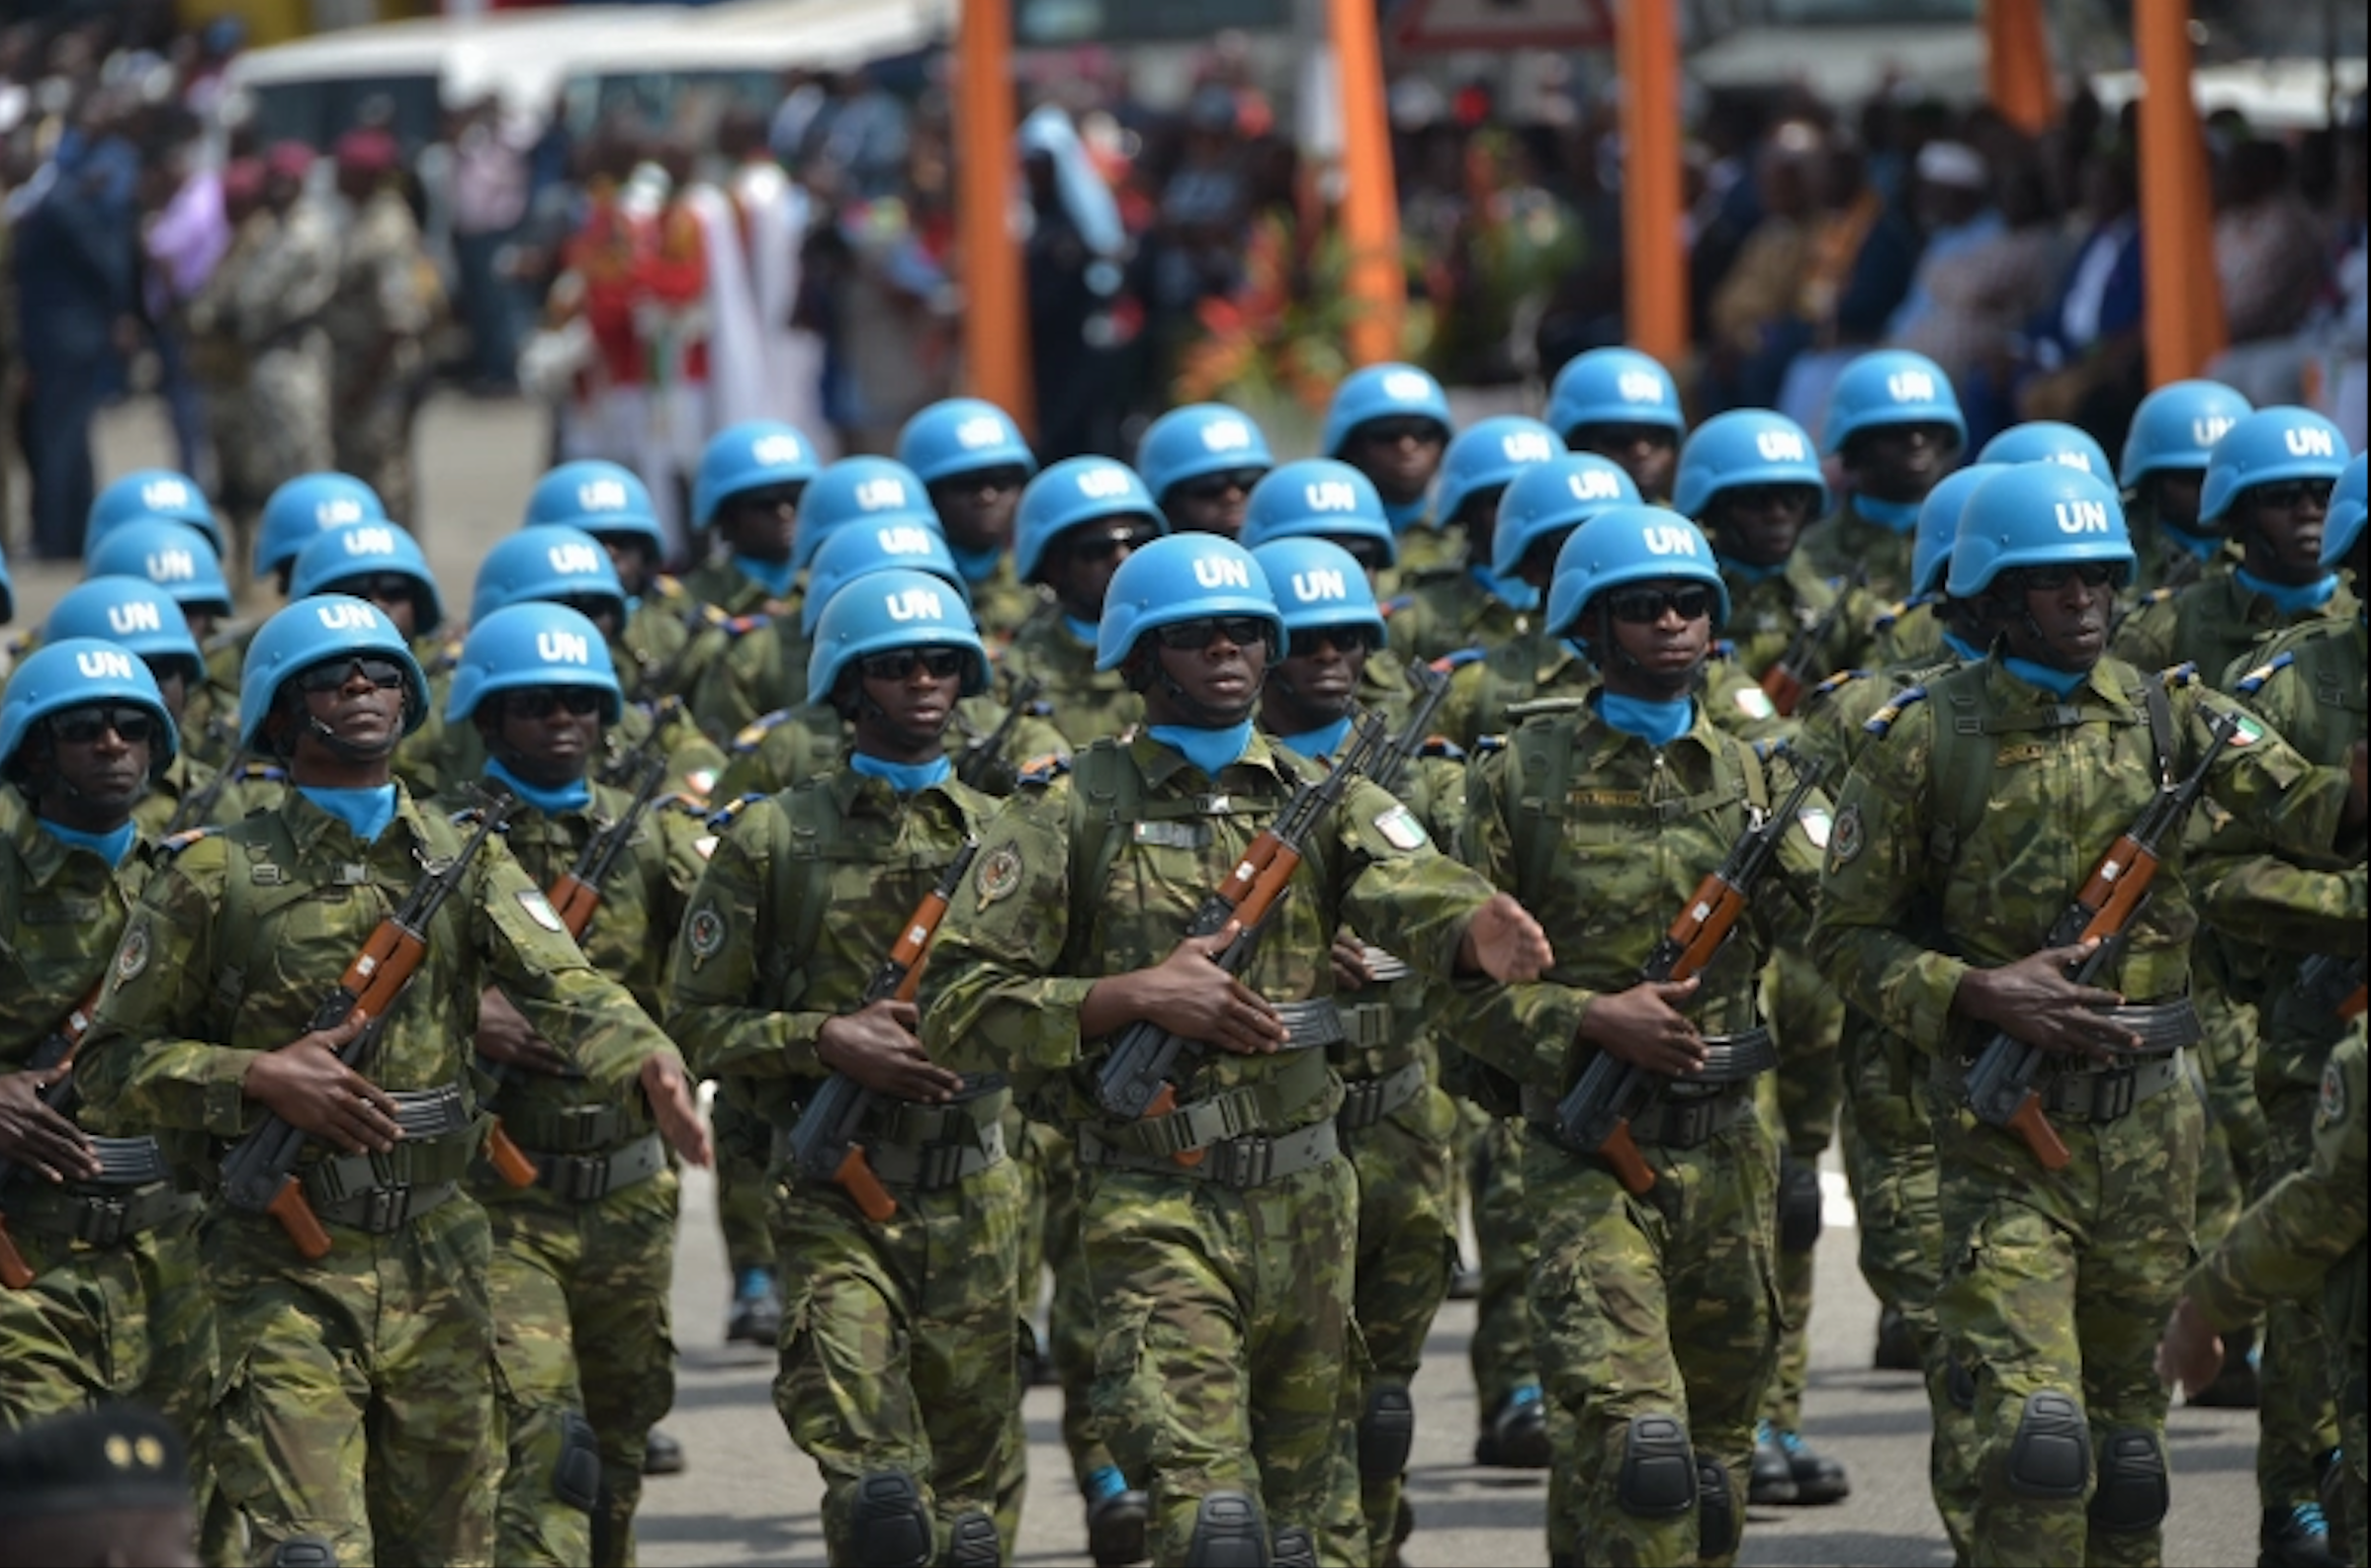
\includegraphics[width=40mm]{Group_Troop.png}
\caption{\scriptsize Peacekeepers in Mali}
\label{Troops}
\end{figure}

\vspace{0.5cm}

\begin{itemize}
  \item \footnotesize Why do troop contributing countries differ in their contribution levels across missions? 
  \pause
  \item \footnotesize Combination of two factors
  \begin{itemize}
    \item \footnotesize Mandate Tasks
    \item \footnotesize Conflict Environment
  \end{itemize}
\end{itemize}
\end{frame}

%%%%%%%%%%%%%%%%%%%%%%%%%%%
\section{Literature Review}
%%%%%%%%%%%%%%%%%%%%%%%%%%%

%%%%%%%%%%%
% Slide 4 %
%%%%%%%%%%%

\begin{frame}
\frametitle{Mission Formation}

\begin{itemize}
  \item United Nations
  \begin{itemize}
    \pause
    \item UNSC forms mandates with tasks
    \pause
    \item Reimbursements and collective action {\tiny (Coleman 2020, Bove 2011)}
    \pause
    \item Flexibility of contributors {\tiny (Leck 2009)}
    \pause
  \end{itemize}
  \item Contribution drivers
  \begin{itemize}
    \pause
    \item Domestic $\rightarrow$ Reimbursements, coup network, regime type {\tiny (Gaibulloev et al. 2015, Kathman and Melin 2017, Duursam and Gledhill 2019)}
    \pause
    \item International $\rightarrow$ Foreign aid, HR ``whitewashing'', kudos {\tiny(Boutton and D'Orazio 2020, Levin 2020, Meiske and Ruggeri 2017)}
  \end{itemize}
  \pause
  \item Lack of mission specific factors
\end{itemize}

\end{frame}


%%%%%%%%%%%
% Slide 5 %
%%%%%%%%%%%

\begin{frame}
\frametitle{Defining Risk}

\begin{itemize}
  \item{Risk to peacekeepers}
  \pause
  \begin{itemize}
    \item Risk of war, terrorist attacks, and post-war mental decomposition {\tiny(Fortna 2008, Hansen et al. 2020, Forbes et al. 2016)}
    \pause
    \item Risk $\rightarrow$ Likelihood of peacekeeper death or injury
  \end{itemize}
\end{itemize}

\end{frame}

%%%%%%%%%%%
% Slide 6 %
%%%%%%%%%%%

\begin{frame}[fragile]

\begin{table}[t]\centering
\def\sym#1{\ifmmode^{#1}\else\(^{#1}\)\fi}
\caption{Table of Task Risk}
\vspace{0.4cm}
\label{Table 1}
\fontsize{5.5}{5.5}\selectfont
\begin{tabular}{c*{2}{c}}
\hline\hline
                    \multicolumn{1}{c}{Risky}         &\multicolumn{1}{c}{Less Risky}      \\
\hline \\
Monitor Peace Agreements                                & Promote Good Offices (Subtask of Monitor Peace Agreements) \\
Subtasks: Buffer Monitor and Liaise War Parties         &  \\
[0.5em]
Monitor Human Rights                                    &   Monitor the Weapons Trade, Monitor Weapons Embargo, \\ 
Subtask: Monitor the Refugee Situation                  & Inspect Cargo (Subtasks of Monitor Borders) \\ 
[0.5em]
Protect Human Rights                                    & Monitor Use of Natural Resources \\
Subtasks: Protect Children, Protect Women,              &  \\
Protect Civilians                                       & \\
[0.5em]
Protect UN Personnel (Ensure Security)                  & Monitor Elections \\
[0.5em]
Assist in Demining                                     & Provide Security During the Electoral Period\\     
[0.5em]
Monitor Borders                                         & Assist with Election Implementation \\
[0.5em]
Chapter VII Authorization                               & Build Government Capacity \\
                                                        & Subtask: Implement Government Policies \\
[0.5em]
Assist with Security Sector Reform                      & Preserve Cultural and Historical Sites \\ 
Subtasks: Assist Police Reform, Monitor the Police,     &   \\
Conduct Joint Patrols with Police                        &   \\ 
[0.5em]
Monitor Disarmament, Demobilization,                    & Assist in the Implementation of Quick Impact Projects (QIP) \\
 and Reintegration                                      & \\
[0.5em]
Help Implement Disarmament, Demobilization,             & Assist with Justice Sector Reform \\ 
and Reintegration                                       & \\
[0.5em]
                                                        & Promote National Reconciliation \\
                                                        & Subtask: Pursue Justice for War Criminals \\
[0.25em]
                                                        & Disseminate Info About the Mission to the Public \\
[0.25em]
                                                        & Promote Freedom of the Press \\                                                                            
\hline\hline
\multicolumn{1}{l}{\fontsize{5}{4}\selectfont Table adapted from tasks coded in Lloyd (2021).}\\

\end{tabular}
\end{table}


\end{frame}


%%%%%%%%%%%%%%%%
\section{Theory}
%%%%%%%%%%%%%%%%

%%%%%%%%%%%
% Slide 7 %
%%%%%%%%%%%

\begin{frame}
\frametitle{State Decisions}

\begin{itemize}
  \pause
  \item Missions go to ``hard cases and places'' {\tiny (Forta 2004, 2008, Gilligan and Stedman 2003, Fjelde et al 2019, Phayal and Prins 2020)}
  \pause
  \item States analyze benefits vs. costs {\tiny (Downs et al 1996, Fearon 1998, Kathman and Melin 2017, Oksamytna et al 2021)}
  \pause
  \item Risk-averse contributors {\tiny (Bove 2011, Page and Stevis 2016, Iwanami 2014)}
  \pause
  \item ``Wars of choice'' {\tiny (Osinga and Lindley-French 2010)}
\end{itemize}

\end{frame}


%%%%%%%%%%%
% Slide 8 %
%%%%%%%%%%%

\begin{frame}
\frametitle{Risky Mandates}

\begin{itemize}
  \pause
  \item Tasks communicate risk of action
  \begin{itemize}
    \pause
    \item Monitor buffer zone {\tiny (Lederer 2017)}
    \item Election security {\tiny (UN-DPPA 2021)}
  \end{itemize}
  \pause
  \item Risky tasks in context of all assigned tasks
  \pause
  \item H1: As the proportion of risky tasks in the mandate \underline{increases}, the number of troops contributed will \underline{decrease}. 
\end{itemize}

\end{frame}

%%%%%%%%%%%
% Slide 9 %
%%%%%%%%%%%

\begin{frame}
\frametitle{Mandates and the Conflict Environment}

\begin{itemize}
  \pause
  \item Tasks communicate risk, but conflict communicates danger
  \begin{itemize}
    \pause
   \item States avoid potential costs {\tiny (Downs et al. 1996)}, but missions move to the danger {\tiny (Phayal and Prins 2020)}
   \item Fear of losing troops {\tiny (Bove 2011)}
   \item Dangerous conditions make risky mandates worse
   \pause
 \end{itemize}
 \item H2: As the level of conflict danger in the mission environment \underline{increases}, the \underline{negative} effect of the proportion of risky tasks in the mandate on the number of troops contributed will \underline{increase}. 
\end{itemize}

\end{frame}

%%%%%%%%%%%%%%%%%%%%%%%%%
\section{Research Design}
%%%%%%%%%%%%%%%%%%%%%%%%%

%%%%%%%%%%%%
% Slide 10 %
%%%%%%%%%%%%

\begin{frame}
\frametitle{The Model}

\begin{itemize}
  \pause
  \item \scriptsize Sample: Contributors and 15 randomly selected potential contributors {\tiny (Savun 2008)}
  \item \scriptsize UoA: Potential-contributor-mission-month, 1990 - 2014
  \pause
  \item \scriptsize DV: Count of troop contributions {\tiny (Perry and Smith 2013)}
  \item \scriptsize IV: Risk ratio {\tiny (Lloyd 2021)}, battle deaths {\tiny (Sundberg and Melander 2013)} 
  \pause
  \item \scriptsize Controls
  \begin{itemize}
    \item \scriptsize Conflict: Conflict outcome and duration {\tiny (Kreutz 2010)}, UN Mission Change, ``Re-hatting" {\tiny (Koops et al. 2015)}
    \item \scriptsize Host: GDP per capita, geographic size, democracy {\tiny (UN Statistics Division 2021, World Bank 2021, Coppedge et al 2021)}
    \item \scriptsize Contributors: GDP per capita, democracy, \# contributors, troop quality, total monthly contributions {\tiny (UN Statistics Division 2021, Coppedge et al 2021, Singer et al 1972)}
    \item \scriptsize Dyad: Same continent, bilateral trade, S-scores {\tiny (Barbieri et al 2009, Chiba et al 2015)}
  \end{itemize}
    \pause
  \item \scriptsize Model: Negative binomial regression, SE's clustered on contributor, lagged IVs, lagged DV
  \item \scriptsize Alternative Specifications: 30 contributors, meta-analysis of 10 samples, same continent and MPs {\tiny (Crescenzi et al. 2011)}, ZINB, include observer missions
\end{itemize}

\end{frame}

%%%%%%%%%%%%
% Slide 11 %
%%%%%%%%%%%%

\begin{frame}
\frametitle{Endogeneity}

\begin{figure}[t]
\centering
\includegraphics[width=70mm]{DAG}
\caption{\scriptsize DAG of Endogeneity}
\label{DAG}
\end{figure}

\end{frame}

%%%%%%%%%%%%%%%%%
\section{Results}
%%%%%%%%%%%%%%%%%

%%%%%%%%%%%%
% Slide 12 %
%%%%%%%%%%%%

\begin{frame}
\frametitle{Testing H1}
\vspace{-4mm}
\begin{figure}[t]
\centering
\includegraphics[width=75mm]{gg_M2_sim_pres.jpg}
\vspace{-5mm}
\caption{\scriptsize Effect of Risk Ratio on Troop Contributions, 95\% CIs}
\label{H1}
\end{figure}

\end{frame}

%%%%%%%%%%%%
% Slide 13 %
%%%%%%%%%%%%

\begin{frame}
\frametitle{Testing H2}
\vspace{-4mm}
\begin{figure}[t]
\centering
\includegraphics[width=75mm]{gg_M3_sim_pres.jpg}
\vspace{-5mm}
\caption{\scriptsize Effect of Risk Ratio and Battle Deaths on Troop Contributions, 95\% CIs}
\label{H2}
\end{figure}

\end{frame}

%%%%%%%%%%%%
% Slide 14 %
%%%%%%%%%%%%

\begin{frame}
\frametitle{Disaggregating Risk Ratio}


\begin{figure}[t]
\centering
\vspace{-5mm}
\includegraphics[width=105mm]{coef.jpg}
\vspace{-4mm}
\caption{\scriptsize Coefficients of Tasks Conditional on Battle Deaths}
\label{Disag}
\end{figure}

\end{frame}

%%%%%%%%%%%%%%%%%%%%
\section{Conclusion}
%%%%%%%%%%%%%%%%%%%%

%%%%%%%%%%%%
% Slide 15 %
%%%%%%%%%%%%

\begin{frame}
\frametitle{Conclusions}


\begin{columns}
% Column 1  
\begin{column}{0.5\textwidth}
    \begin{figure}
    \centering
        \includegraphics[width=1\textwidth]{mandate}
        \caption{Peacekeeper Receives Medal}
    \end{figure}
\end{column}
% Column 2  
\begin{column}{0.5\textwidth}
        \begin{itemize}
        \pause
        \item States are deterred by mandate risk.
        \item Further deterred by conflict conditions. 
        \item ``Risky" tasks differ in direction.
        \pause
        \item Future work
        \begin{itemize}
          \item Higher risk, more ``whitewashed''
          \item More risk, more foreign aid needed 
        \end{itemize}
        \end{itemize}
\end{column}
\end{columns}

\end{frame}

%%%%%%%%%%%%
% Slide 16 %
%%%%%%%%%%%%

\begin{frame}
\frametitle{Thank You}

\centering
\begin{itemize}
\item Please reach out!
\item trey.wood@uky.edu
\end{itemize}
\end{frame}

%%%%%%%%%%%%%%%%%%
\section{Appendix}
%%%%%%%%%%%%%%%%%%

%%%%%%%%%%%%
% Slide 17 %
%%%%%%%%%%%%

\begin{frame}
\frametitle{Distribution of DV}

\begin{figure}
\centering
\begin{minipage}{.5\textwidth}
  \centering
  \includegraphics[width=.90\linewidth]{gg_Hist_DV.jpg}
  \caption{Histogram of Troops}
  \label{fig:test1}
\end{minipage}%
\begin{minipage}{.5\textwidth}
  \centering
  \includegraphics[width=.90\linewidth]{gg_Hist_DV_No_0.jpg}
  \caption{Histogram of Troops, No 0's}
  \label{fig:test2}
\end{minipage}
\end{figure}

\end{frame}

%%%%%%%%%%%%
% Slide 18 %
%%%%%%%%%%%%

\begin{frame}
\frametitle{Distribution of IV}

\begin{figure}[t]
\centering
\includegraphics[width=65mm]{gg_Hist_RR_lab.jpg}
\caption{\scriptsize Distribution of IV iwth Example Missions}
\label{H1}
\end{figure}

\end{frame}

%%%%%%%%%%%%
% Slide 19 %
%%%%%%%%%%%%

\begin{frame}[fragile]
\frametitle{Main Model Output}

\begin{table}[htbp]\centering
\tiny
\def\sym#1{\ifmmode^{#1}\else\(^{#1}\)\fi}
\caption{The Effect of Risk Ratio on Contributions \label{Table 2}}
\vspace{0.4cm}
\begin{tabular}{l*{3}{c}}
\hline\hline
                    &\multicolumn{1}{c}{(1)}        &\multicolumn{1}{c}{(2)}        &\multicolumn{1}{c}{(3)}        \\
                    &          Model 1        &          Model 2        &          Model 3        \\
\hline
Risk Ratio$_{t-1}$          &      -1.439\sym{**}&      -1.646\sym{**}&      -1.460\sym{**}\\
                    &     (0.457)        &     (0.373)        &     (0.406)        \\
[1em]
Battle Deaths$_{t-1}$ (Hundreds)&     -0.0124        &     -0.0588        &       0.883\sym{*} \\
                    &    (0.0941)        &    (0.0784)        &     (0.419)        \\
[1em]
Risk Ratio$_{t-1}$ X Battle Deaths$_{t-1}$&                    &                    &      -1.198\sym{*} \\
                    &                    &                    &     (0.537)        \\
[1em]
Controls?           &       NO          &        YES         &         YES        \\
[1em]
Constant            &       3.321\sym{**}&       2.201\sym{**}&       2.030\sym{**}\\
                    &     (0.376)        &     (0.487)        &     (0.493)        \\
\hline
lnalpha             &       1.997\sym{**}&       1.841\sym{**}&       1.841\sym{**}\\
                    &    (0.0801)        &    (0.0739)        &    (0.0739)        \\
\hline
Observations        &       79107        &       72292        &       72292        \\
\hline\hline
\multicolumn{4}{l}{\tiny Contributing state clustered standard errors in parentheses}\\
\multicolumn{4}{l}{\tiny Dependent variable is troop counts. 15 potential contributor random sample.}\\
\multicolumn{4}{l}{\tiny \sym{\dagger} \(p<0.10\), \sym{*} \(p<0.05\), \sym{**} \(p<0.01\)}\\
\end{tabular}
\end{table}

\end{frame}


%%%%%%%%%%%%
% Slide 20 %
%%%%%%%%%%%%

\begin{frame}[fragile]

\begin{table}[htbp]\centering
\fontsize{5.5}{6}\selectfont
\def\sym#1{\ifmmode^{#1}\else\(^{#1}\)\fi}
\caption{Meta Analysis of 10 Random Samples \label{Table 10}}
\vspace{0.4cm}
\begin{tabular}{l*{4}{c}}
\hline\hline
        &\multicolumn{1}{c}{(1)}     &\multicolumn{1}{c}{(2)}  & \multicolumn{1}{c}{(3)}  & \multicolumn{1}{c}{(4)}      \\
        &          15                &          30             & 15 with Interaction      & 30 with Interaction         \\
\hline
Risk Ratio$_{t-1}$ &   -1.648        &      -1.724        &    -1.464           &   -1.497   \\
                 &  [-1.882, -1.415]  &   [-2.014, -1.435] &  [-1.718, -1.210]   &  [-1.805, -1.189]  \\
[0.25em]
Battle Deaths$_{t-1}$ (Hundreds)  &         &             &     0.867           &  1.303  \\
        &                           &                     &  [0.616, 1.136]     & [0.991, 1.615] \\
[0.25em]
Risk Ratio$_{t-1}$ X Battle Deaths$_{t-1}$  &   &         &   -1.186            &   -1.693 \\
                    &               &                     &   [-1.518, -0.853]  &   [-2.074, -1.312] \\ 
\hline\hline
\multicolumn{5}{l}{\fontsize{5.5}{6}\selectfont 95\% Confidence intervals presented in brackets.}\\
\multicolumn{5}{l}{\fontsize{5.5}{6}\selectfont Dependent variable is troop counts. Common effect model with inverse-variance.}\\
\multicolumn{5}{l}{\fontsize{5.5}{6}\selectfont Read as overall effect size across all 10 random samples.}\\
\end{tabular}
\end{table}

\end{frame}



%%%%%%%%%%%%
% Slide 21 %
%%%%%%%%%%%%

\begin{frame}[fragile]
\frametitle{All Battle Deaths}

\begin{table}[htbp]\centering
\tiny
\def\sym#1{\ifmmode^{#1}\else\(^{#1}\)\fi}
\caption{The Effect of Risk Ratio on Contributions without Battle Death Restrictions \label{Table 5}}
\vspace{0.4cm}
\begin{tabular}{l*{2}{c}}
\hline\hline
                    &\multicolumn{1}{c}{(1)}        &\multicolumn{1}{c}{(2)}        \\
                    &          Model 4        &          Model 5       \\
\hline
Risk Ratio$_{t-1}$          &      -1.640\sym{**}&      -1.623\sym{**}\\
                    &     (0.360)        &     (0.360)        \\
[1em]
Risk Ratio$_{t-1}$ X Battle Deaths$_{t-1}$ &                    &     -0.0202\sym{*} \\
                    &                    &   (0.00866)        \\
[1em]
Battle Deaths$_{t-1}$ (Hundreds)&    0.000171        &      0.0201\sym{*} \\
                    &  (0.000342)        &   (0.00871)        \\
[1em]
Controls?           &         YES        &         YES        \\
[1em]
Constant            &       2.215\sym{**}&       2.189\sym{**}\\
                    &     (0.486)        &     (0.489)        \\
\hline
lnalpha             &       1.831\sym{**}&       1.831\sym{**}\\
                    &    (0.0732)        &    (0.0731)        \\
\hline
Observations        &       78848        &       78848        \\
\hline\hline
\multicolumn{3}{l}{\tiny Contributing state clustered standard errors in parentheses.}\\
\multicolumn{3}{l}{\tiny Dependent variable is troop counts. 15 potential contributor random sample. No battle death restriction.}\\
\multicolumn{3}{l}{\tiny \sym{\dagger} \(p<0.10\), \sym{*} \(p<0.05\), \sym{**} \(p<0.01\)}\\
\end{tabular}
\end{table}

\end{frame}

%%%%%%%%%%%%
% Slide 22 %
%%%%%%%%%%%%

\begin{frame}[fragile]
\frametitle{With Observer Missions}

\begin{table}[htbp]\centering
\tiny
\def\sym#1{\ifmmode^{#1}\else\(^{#1}\)\fi}
\caption{The Effect of Risk Ratio on Contributions with Observer Missions \label{Table 6}}
\vspace{0.4cm}
\begin{tabular}{l*{2}{c}}
\hline\hline
                    &\multicolumn{1}{c}{(1)}        &\multicolumn{1}{c}{(2)}        \\
                    &          Model 6        &          Model 7        \\
\hline
Risk Ratio$_{t-1}$          &      -1.151\sym{**}&      -0.919\sym{*} \\
                    &     (0.425)        &     (0.444)        \\
[1em]
Battle Deaths$_{t-1}$ (Hundreds)&     -0.0588        &       1.402\sym{**}\\
                    &    (0.0929)        &     (0.409)        \\
[1em]
Risk Ratio$_{t-1}$ X Battle Deaths$_{t-1}$ &                    &      -1.850\sym{**}\\
                    &                    &     (0.498)        \\
[1em]
Controls?           &        YES         &         YES        \\
[1em]
Constant            &       1.435\sym{**}&       1.249\sym{*} \\
                    &     (0.504)        &     (0.501)        \\
\hline
lnalpha             &       1.989\sym{**}&       1.988\sym{**}\\
                    &    (0.0741)        &    (0.0741)        \\
\hline
Observations        &       84842        &       84842        \\
\hline\hline
\multicolumn{3}{l}{\tiny Contributing state clustered standard errors in parentheses.}\\
\multicolumn{3}{l}{\tiny Dependent variable is troop counts. 15 potential contributor random sample. Inclusion of observer missions.}\\
\multicolumn{3}{l}{\tiny \sym{\dagger} \(p<0.10\), \sym{*} \(p<0.05\), \sym{**} \(p<0.01\)}\\
\end{tabular}
\end{table}

\end{frame}


%%%%%%%%%%%%
% Slide 23 %
%%%%%%%%%%%%

\begin{frame}[fragile]
\frametitle{30 Potential Contributors}

\begin{table}[htbp]\centering
\tiny
\def\sym#1{\ifmmode^{#1}\else\(^{#1}\)\fi}
\caption{The Effect of Risk Ratio on Contributions with 30 Potential Contributors \label{Table 7}}
\vspace{0.4cm}
\begin{tabular}{l*{2}{c}}
\hline\hline
                    &\multicolumn{1}{c}{(1)}        &\multicolumn{1}{c}{(2)}        \\
                    &          Model 8        &          Model 9        \\
\hline
Risk Ratio$_{t-1}$          &      -1.731\sym{**}&      -1.501\sym{**}\\
                    &     (0.466)        &     (0.496)        \\
[1em]
Battle Deaths$_{t-1}$ (Hundreds)&     -0.0385        &       1.311\sym{**}\\
                    &     (0.105)        &     (0.500)        \\
[1em]
Risk Ratio$_{t-1}$ X Battle Deaths$_{t-1}$&                    &      -1.708\sym{**}\\
                    &                    &     (0.610)        \\
[1em]
Controls?           &        YES         &        YES         \\
[1em]
Constant            &       0.924\sym{\dagger} &       0.709        \\
                    &     (0.523)        &     (0.531)        \\
\hline
lnalpha             &       2.297\sym{**}&       2.296\sym{**}\\
                    &    (0.0804)        &    (0.0803)        \\
\hline
Observations        &      108357        &      108357        \\
\hline\hline
\multicolumn{3}{l}{\tiny Contributing state clustered standard errors in parentheses.}\\
\multicolumn{3}{l}{\tiny Dependent variable is troop counts. 30 potential contributor random sample.}\\
\multicolumn{3}{l}{\tiny \sym{\dagger} \(p<0.10\), \sym{*} \(p<0.05\), \sym{**} \(p<0.01\)}\\
\end{tabular}
\end{table}

\end{frame}

%%%%%%%%%%%%
% Slide 24 %
%%%%%%%%%%%%

\begin{frame}[fragile]
\frametitle{Same Continent, Major Powers Sample}

\begin{table}[htbp]\centering
\tiny
\def\sym#1{\ifmmode^{#1}\else\(^{#1}\)\fi}
\caption{The Effect of Risk Ratio on Contributions with Same Continent and Major Power Sample \label{Table 7}}
\vspace{0.4cm}
\begin{tabular}{l*{2}{c}}
\hline\hline
                    &\multicolumn{1}{c}{(1)}        &\multicolumn{1}{c}{(2)}        \\
                    &          Model 10        &         Model 11        \\
\hline
Risk Ratio$_{t-1}$          &      -2.171\sym{**}&      -2.125\sym{**}\\
                    &     (0.498)        &     (0.525)        \\
[1em]
Battle Deaths$_{t-1}$ (Hundreds)&      0.0705        &       0.411        \\
                    &     (0.118)        &     (0.605)        \\
[1em]
Risk Ratio$_{t-1}$ X Battle Deaths$_{t-1}$ &                    &      -0.435        \\
                    &                    &     (0.767)        \\
Controls?           &         YES        &        YES         \\
[1em]
Constant            &       2.889\sym{**}&       2.848\sym{**}\\
                    &     (0.604)        &     (0.629)        \\
\hline
lnalpha             &       2.419\sym{**}&       2.419\sym{**}\\
                    &    (0.0986)        &    (0.0986)        \\
\hline
Observations        &      125249        &      125249        \\
\hline\hline
\multicolumn{3}{l}{\tiny Contributing state clustered standard errors in parentheses.}\\
\multicolumn{3}{l}{\tiny Dependent variable is troop counts. Same continent and major power sample.}\\
\multicolumn{3}{l}{\tiny \sym{\dagger} \(p<0.10\), \sym{*} \(p<0.05\), \sym{**} \(p<0.01\)}\\
\end{tabular}
\end{table}

\end{frame}

%%%%%%%%%%%%
% Slide 25 %
%%%%%%%%%%%%

\begin{frame}[fragile]
\frametitle{Conflict Dynamics and Risk}

\begin{table}[htbp]\centering
\fontsize{5}{6}\selectfont
\def\sym#1{\ifmmode^{#1}\else\(^{#1}\)\fi}
\caption{Predicting Mandate Risk with Conflict Dynamics\label{Fraq}}
\vspace{0.4cm}
\begin{tabular}{l*{2}{c}}
\hline\hline
                    &\multicolumn{1}{c}{(1)}        &\multicolumn{1}{c}{(2)}        \\
                    &         Model 12        &         Model 13        \\
\hline
Battle Deaths$_{t-1}$ (Hundreds)&    0.000718        &      0.0929        \\
                    &     (0.281)        &     (0.125)        \\
[0.25em]
Conflict Termination$_{t-1}$&                    &       0.812\sym{\dagger} \\
                    &                    &     (0.420)        \\
[0.25em]
Low Activity$_{t-1}$        &                    &       0.472        \\
                    &                    &     (0.351)        \\
[0.25em]
Conflict Duration$_{t-1}$ (Logged)&                    &      -0.453\sym{*} \\
                    &                    &     (0.187)        \\
[0.25em]
Previous UN Mission$_{t-1}$ &                    &       0.332        \\
                    &                    &     (0.357)        \\
[0.25em]
Re-hatted$_{t-1}$           &                    &      -0.170        \\
                    &                    &     (0.327)        \\
[0.25em]
Host GDP per Capita$_{t-1}$ (Thousands)&                    &       0.315\sym{**}\\
                    &                    &    (0.0583)        \\
[0.25em]
Host Size$_{t-1}$ (Million Sq. Km)&                    &      0.0654        \\
                    &                    &     (0.200)        \\
[0.25em]
Host Democracy$_{t-1}$      &                    &      -1.868\sym{*} \\
                    &                    &     (0.919)        \\
[0.25em]
Constant            &       1.399\sym{**}&       1.539\sym{**}\\
                    &     (0.301)        &     (0.532)        \\
\hline
Observations        &        2824        &        2796        \\
\hline\hline
\multicolumn{3}{l}{\fontsize{5}{6}\selectfont Mission clustered standard errors in parentheses}\\
\multicolumn{3}{l}{\fontsize{5}{6}\selectfont Dependent variable is risk ratio. Standard errors clustered on the mission.}\\
\multicolumn{3}{l}{\fontsize{5}{6}\selectfont \sym{\dagger} \(p<0.10\), \sym{*} \(p<0.05\), \sym{**} \(p<0.01\)}\\
\end{tabular}
\end{table}

\end{frame}

%%%%%%%%%%%%
% Slide 26 %
%%%%%%%%%%%%

\begin{frame}[fragile]
\frametitle{Zero Inflated Models}

\begin{table}[htbp]\centering
\tiny
\def\sym#1{\ifmmode^{#1}\else\(^{#1}\)\fi}
\caption{The Effect of Risk Ratio on Contributions, Zero Inflated Models}
\vspace{0.4cm}
\begin{tabular}{l*{2}{c}}
\hline\hline
                    &\multicolumn{1}{c}{(1)}        &\multicolumn{1}{c}{(2)}        \\
                    &         Model 14        &         Model 15        \\
\hline
Risk Ratio          &      -1.593\sym{**}&      -1.355\sym{*} \\
                    &     (0.515)        &     (0.532)        \\
[1em]
Battle Deaths (Hundreds)&     -0.0565        &       1.164\sym{*} \\
                    &     (0.106)        &     (0.491)        \\
[1em]
Risk Ratio $\times$ Battle Deaths (Hundreds)&                    &      -1.548\sym{*} \\
                    &                    &     (0.602)        \\
[1em]
Controls for Count? &     YES            &       YES          \\
[1em]
Controls for Inflation? &        YES     &       YES          \\
[1em]
lnalpha             &       3.193\sym{**}&       3.193\sym{**}\\
                    &    (0.0928)        &    (0.0928)        \\
\hline
Observations        &      473552        &      473552        \\
\hline\hline
\multicolumn{3}{l}{\tiny Contributing state clustered standard errors in parentheses}\\
\multicolumn{3}{l}{\tiny Dependent variables is troop counts. Zero-inflated negative biomial regression.}\\
\multicolumn{3}{l}{\tiny \sym{\dagger} \(p<0.10\), \sym{*} \(p<0.05\), \sym{**} \(p<0.01\)}\\
\end{tabular}
\end{table}

\end{frame}


\end{document}